%% LyX 2.1.4 created this file.  For more info, see http://www.lyx.org/.
%% Do not edit unless you really know what you are doing.
\documentclass[oneside,english]{amsart}
\usepackage[T1]{fontenc}
\usepackage[latin9]{inputenc}
\usepackage[landscape]{geometry}
\geometry{verbose,tmargin=0.5in,bmargin=0.5in,lmargin=0.5in,rmargin=0.5in}
\setlength{\parskip}{\smallskipamount}
\setlength{\parindent}{0pt}
\usepackage{array}
\usepackage{float}
\usepackage{calc}
\usepackage{multirow}
\usepackage{amsthm}
\usepackage{amssymb}

\makeatletter

%%%%%%%%%%%%%%%%%%%%%%%%%%%%%% LyX specific LaTeX commands.
%% Because html converters don't know tabularnewline
\providecommand{\tabularnewline}{\\}

%%%%%%%%%%%%%%%%%%%%%%%%%%%%%% Textclass specific LaTeX commands.
\numberwithin{equation}{section}
\numberwithin{figure}{section}
\usepackage{enumitem}		% customizable list environments
\newlength{\lyxlabelwidth}      % auxiliary length 

%%%%%%%%%%%%%%%%%%%%%%%%%%%%%% User specified LaTeX commands.
\usepackage{hyperref}
\usepackage[usenames,dvipsnames,table]{xcolor} %adds additional color options
\hypersetup{colorlinks=true, urlcolor=black,linkcolor=black}

\usepackage{fancyhdr}
\usepackage{lastpage}
\pagestyle{fancy}
\usepackage{enumitem}
\usepackage{ifthen}
%sets math fonts to be more readable
\everymath=\expandafter{\the\everymath\displaystyle}
\DeclareMathSizes{10}{10}{10}{10}
\usepackage{multicol}

\usepackage{tikz}
\usepackage{tikz-3dplot}
\usetikzlibrary{shapes,calc,positioning}
\usepackage{tkz-euclide} %%angle marks and such
%%prevents unnecessary whitespace cretead in projection
\makeatletter
\def\tkz@Projection(#1,#2)(#3)#4{%
\begingroup 
  \pgfpointdiff{\pgfpointanchor{#1}{center}}%
               {\pgfpointanchor{#2}{center}}%
  \tkz@ax =\pgf@y%
  \tkz@ay =\pgf@x%
  \begin{pgfinterruptboundingbox}
  \path[coordinate](#3)--++(-\tkz@ax,\tkz@ay) coordinate (tkz@point);
  \end{pgfinterruptboundingbox}
  \tkz@InterLL(#1,#2)(#3,tkz@point){#4}% définit tkzPointResult 
\endgroup
}
\makeatother
%%%%%%%%%%%%%%%%%%
\usetikzlibrary{patterns} % replaces obsolete usetkzobj (tkz-euclide 3+)
\usetikzlibrary{plotmarks}
\usepackage{pgfplots}
\pgfplotsset{compat=newest}
\usepackage{pgf-pie}
\usepackage{pstricks,pst-plot}
\usepackage{calc}
%%\usepackage[nomessages]{fp} clashes with tkz-euclide?

%\usepackage{advdate}    % Advancing/saving dates
\usepackage{datetime}   % Dates formatting
%\usepackage{datenumber} % Counters for dates
\newdateformat{MD}{\monthname[\THEMONTH] \ordinal{DAY}}

\def\formatdateny{\csname noyear\languagename\expandafter\endcsname\formatdate}
\def\noyearenglish#1, \the\@year{#1}
\let\noyearamerican\noyearenglish
\let\noyearbritish\noyearenglish

\usepackage{fancybox} %%ovalbox and fancy box settings

\usepackage[outline]{contour}  %allows text halos
\usepackage{colortbl}


\usepackage[super]{nth} %easy 1st, 2nd, etc

\usepackage{forest} %%for tree diagram
\usepackage{caption}%%allows turing off numbers on fig
\usepackage{subcaption}
\makeatletter %%to fix LyX error?

\makeatother

\usepackage{babel}
\begin{document}
\renewcommand{\author}{WGU Math Center}

\newcommand{\classNum}{}

\newcommand{\classSec}{}

\newcommand{\nameType}{}

\newcommand{\examType}{Praxis 5001 Practice Exam Version 2: Math (5003)}

\renewcommand{\date}{\today}

%%First page's header%%%%%%%%%%%%%%%%%%%%%%
\fancypagestyle{firststyle} %%header settings for first pagr
{
	\fancyhead[L]{\author}
	\fancyhead[C]{\textbf{\examType}}
	%\fancyhead[R]{\date}
	\setlength{\headsep}{30pt}

head{}
	\lfoot{\date}
}
%%%%%%%%%%%%%%%%%%%%%%%%%%%%%%%%%%%%%%%%%%

%%Next page's header%%%%%%%%%%%%%%%%%%%%%%%
%\setlist{nolistsep}
\lhead{\author} 
\chead{\textbf{\examType}}
\cfoot{\thepage{}~of~\pageref{LastPage}} 

head{}

\setlength{\headsep}{30pt}

%%%%%%%%%%%%%%%%%%%%%%%%%%%%%%%%%%%%%%%%%%%%%Various settings; see the preamble for other settings%%%%%
%%\setenumerate[0]{leftmargin=12pt,itemindent=0pt,labelwidth=0pt}
%\setlist[2]{noitemsep}
%\setlist{nosep}
\setlist{itemsep=8pt,topsep=12pt} %,parsep=0pt}
\setlength\multicolsep{3pt}
\setlength{\parindent}{0pt} %%no indent
\renewcommand{\labelenumi}{\textbf{\arabic{enumi}.}}
\renewcommand{\labelenumii}{\textbf{\alph{enumii}.}}
\thispagestyle{firststyle}

%%%%%%For problem type%%%%%%%%%%%%%%%%%%%%
%\newcommand{\clicking}{\textbf{clicking on}~}
\newcommand{\clicking}{\textbf{choosing}~}
%\newcommand{\click}{\textbf{~Click on~}}
\newcommand{\click}{\textbf{~Indicate all~}}

\setenumerate[2]{label=\textbf{\Alph*.}}%%%changes enumii to capital letters 

\newcommand{\questMulti}{\renewcommand\labelitemi{\myEllipse} \textbf{Answer the question below by }\clicking\textbf{the correct response.} \\ \\~}

\newcommand{\questMultiPic}{\renewcommand\labelitemi{\myEllipse} \textbf{Answer the question below by }\clicking\textbf{the correct response.}}

\newcommand{\questFill}{\textbf{Write your answer in the provided form.} \\ \\}

\newcommand{\questFillPic}{\textbf{Write your answer in the provided form.}}

\newcommand{\questInd}{\renewcommand\labelitemi{\myBox}  \textbf{Indicate all of your answers.} \\ \\}
   
%%%%%%%%%%%%%%%%%%%%%%%%%%%%%%%%%%%%%%%%%%
\newcommand{\xmax}{10}
\newcommand{\xmin}{-10}
\newcommand{\xstep}{0} %must be xmin+n
\newcommand{\ymax}{10}
\newcommand{\ymin}{-10}
\newcommand{\ystep}{0} %must be ymin+n

%%comments%%
\definecolor{readablegreen}{rgb}{0,0.4,0}

%%%picture macros and settings%%%
\newcommand{\gWidth}{6cm}
\newcommand{\gHeight}{6cm} 
\newcommand{\Scale}{1.0} 
\newcommand{\textSize}{\normalsize} 
\pgfplotsset{minor grid style={white!35!black}} %%changes gridline style
\pgfplotsset{major grid style={white!35!black}}

%%%options%%
%\tiny \scriptsize \footnotesize \small \normalsize, \large, \Large, \LARGE, \huge, \Huge
\newcommand{\examTextSize}{\LARGE} %text size
\examTextSize %%set size
\newcommand{\multi}{\cdot}
\newcommand{\xspace}{\hspace*{0pt}}
\newcommand{\yspace}{\vspace{0pt} \newpage} %1.4cm

%%%for bubbles and boxes%%%%%
\newcommand*{\ansEllipse}{ 	
	\begin{tikzpicture} 		
	\draw[black,thick, fill=readablegreen] (0,0) ellipse (.35cm and .185cm); 	
	\end{tikzpicture} 	
	} 

\newcommand*{\myEllipse}{
	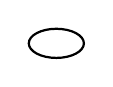
\begin{tikzpicture}
		\draw[thick] (0,0) ellipse (.35cm and .185cm);
	\end{tikzpicture}
	}

\newcommand*{\ansBox}{
	\begin{tikzpicture}
		\draw[thick,fill=readablegreen] (0,0) rectangle (.325,.325);
	\end{tikzpicture}
	}

\newcommand*{\myBox}{ 	
	
\begin{tikzpicture} 		
		\draw[thick] (0,0) rectangle (.325,.325);
	\end{tikzpicture}
	}

%%%%%Answers%%%%%%%%%%%%%%%%%%%%%%%%%%%%%%%%%%%%%%%%%%%%
%%%%%\quest micros set labelitemi for boxes or ovals%%%%
%%Turn answers off/on by uncommenting/commenting renewcommands%%%
\newcommand{\ans}{\textcolor{readablegreen}{\textbf{\checkmark}}}
\renewcommand{\ans}{}
%\newcommand{\ansE}{\ansEllipse}
\newcommand{\ansE}{\ans}
%\newcommand{\ansB}{\ansBox}
\newcommand{\ansB}{\ans}
\newcommand{\answer}[1]{\textbf{\textcolor{readablegreen}{#1}}} 
%\renewcommand{\ansE}{\myEllipse}
\renewcommand{\ansE}{\ans}
%\renewcommand{\ansB}{\myBox}
\renewcommand{\ansB}{\ans}
\renewcommand{\answer}[1]{\textbf{\textcolor{white}{#1}}}

%%%options%%
\renewcommand{\textSize}{\tiny}
\renewcommand{\textSize}{\normalsize}
%%\tiny \scriptsize \footnotesize \small \normalsize, \large, \Large, \LARGE, \huge, \Huge
\renewcommand{\examTextSize}{\small}
\renewcommand{\examTextSize}{\LARGE}
\examTextSize
\renewcommand{\multi}{\cdot}
\renewcommand{\xspace}{\hspace*{0pt}}
\renewcommand{\yspace}{\vspace{0pt} \vfill} %1.4cm
\renewcommand{\yspace}{\vspace{0pt} \newpage} %1.4cm
\begin{enumerate}[resume]
\item \questMulti Which of the following is the expanded form of 4,307.67?

\begin{enumerate}
\item $\left(4\times\mbox{1,000}\right)+\left(3\times100\right)+\left(7\times1\right)+\left(6\times\frac{1}{100}\right)+\left(7\times\frac{1}{10}\right)$
\item  \ans $\left(4\times\mbox{1,000}\right)+\left(3\times100\right)+\left(7\times1\right)+\left(6\times\frac{1}{10}\right)+\left(7\times\frac{1}{100}\right)$
\item $\left(4\times\mbox{1,000}\right)+\left(3\times100\right)+\left(7\times10\right)+\left(6\times\frac{1}{10}\right)+\left(7\times\frac{1}{100}\right)$
\item $\left(4\times\mbox{1,000}\right)+\left(3\times100\right)+\left(7\times10\right)+\left(6\times1\right)+\left(7\times\frac{1}{100}\right)$\yspace \vfill
\end{enumerate}
\item \questMulti Hugh needs to fill milk jugs to take to sell to a grocery
market. The number of jugs, $n$, needed to fill the order is $n=3w+2$,
where \emph{$w$} is the number of weeks until the next delivery.\\
\\
Which of the following statements is true about the variables \emph{$n$
}and $w$?

\begin{enumerate}
\item $n$ is the independent variable, and $w$ is the dependent variable.
\item  \ans $w$ is the independent variable, and $n$ is the dependent
variable.
\item Both $n$ and $w$ are dependent variables.
\item Both $n$ and $w$ are independent variables.\yspace \vfill
\end{enumerate}
\item \questMulti Tiana has $T$ tiaras, and Cinderella has $C$ tiaras.
If Tiana has three times as many tiaras as Cinderella and together
they have a total of 40 tiaras, which of the following proportions
can be used to find out how many tiaras Tiana has?

\begin{enumerate}
\item $T\,\colon C=3\,\colon4$
\item $C\,\colon T=3\,\colon4$
\item  \ans $T\,\colon\left(C+T\right)=3\,\colon4$
\item $C\,\colon\left(C+T\right)=3\,\colon4$\yspace \vfill
\end{enumerate}
\item \questMultiPic 
\begin{figure}[H]
\begin{center}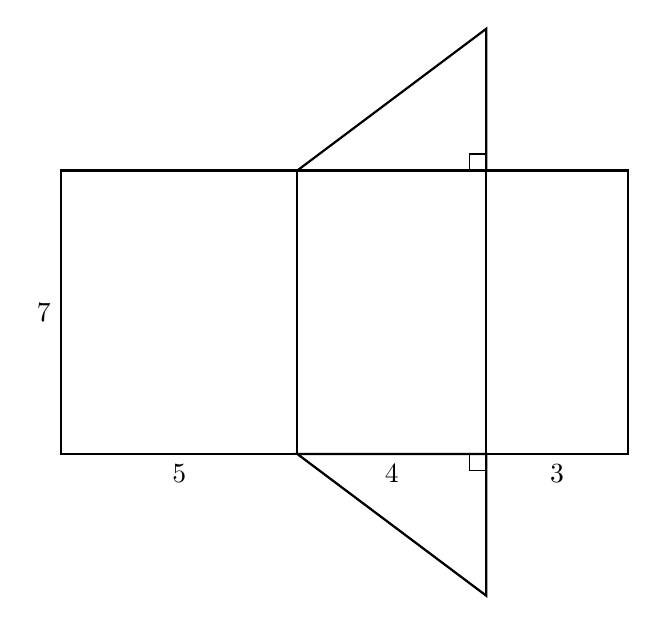
\begin{tikzpicture}[scale=0.6]
	\def\Wa{5};
	\def\Wb{4};
	\def\Wc{3}; %%widths of three sides; they need to form a right triangle
	\def\Ha{6}; %%height of prism
	
	%%bottom of rectangles
	\coordinate (A) at (0,0);
	\coordinate (B) at (\Wa,0);	
	\coordinate (C) at (\Wa + \Wb,0); 	
	\coordinate (D) at (\Wa +\Wb + \Wc,0);
	%%top of rectangles
	\coordinate (E) at (\Wa +\Wb +\Wc,\Ha);
	\coordinate (F) at (\Wa +\Wb,\Ha); 	
	\coordinate (G) at (\Wa,\Ha);	
	\coordinate (H) at (0,\Ha);
	%%%triangle "tops"
	\coordinate (I) at (\Wa +\Wb,-\Wc);
	\coordinate (J) at (\Wa +\Wb,\Ha +\Wc);
	
	%%Big rectangle%%
	\draw[thick] (A)--(B) node[below,pos=.5] {$\Wa$} 
		--(C) node[below,pos=.5] {$\Wb$}
		--(D) node[below,pos=.5] {$\Wc$}
		--(E)--(F)--(G)--(H)
		--cycle node[left,pos=.5] {$7$};
	%%little rectangles%%
	\draw[thick] (B)--(G); \draw[thick] (C)--(F);
	%%triangles%%
	\draw[thick] (B)--(C)--(I)--cycle;	
		\tkzMarkRightAngle[size=0.35,opacity=1](B,C,I)
	\draw[thick] (F)--(G)--(J)--cycle;	
		\tkzMarkRightAngle[size=0.35,opacity=1](G,F,J)

\end{tikzpicture}\end{center}
\end{figure}
\noindent The net shown above forms a right triangular prism. Which
of the following is the surface area of the right triangular prism
in square units?

\begin{enumerate}
\item 84 
\item  \ans 96
\item 108
\item 120\yspace \vfill
\end{enumerate}
\item \questMultiPic 
\begin{figure}[H]
\begin{center}%
\begin{tabular}{|c|c|c|}
\hline 
Item & ~Cost per Package~ & ~~~\tabularnewline
\hline 
Pens & \$2.50 & 4\tabularnewline
\hline 
Pencils & \$2.00 & 6\tabularnewline
\hline 
Staples & \$2.00 & 2\tabularnewline
\hline 
~Notebooks~ & \$3.50 & 2\tabularnewline
\hline 
\end{tabular}\end{center}
\end{figure}
\noindent The table above shows the costs of office supplies. Andy
buys 4 packages of pens, 6 packages of pencils, 2 boxes of staples,
and 2 boxes of notebooks. Andy also has to pay 5\% sales tax. How
much will the supplies cost?

\begin{enumerate}
\item \$10.00
\item \$10.50
\item \$33.00
\item  \ans \$34.65\yspace \vfill
\end{enumerate}
\item \questMultiPic  
\begin{figure}[H]
\begin{center}%
\fbox{\begin{minipage}[t]{0.55\textwidth}%
A box contains $B$ books and $M$ magazines, and there are three
fewer books than twice the number of magazines. %
\end{minipage}} \end{center}
\end{figure}
\noindent Which of the following equations can be used to represent
algebraically the relationship between the number of books and the
number of magazines in the box?

\begin{enumerate}
\item $B=3-2M$
\item $B-3=2M$
\item  \ans $B+3=2M$
\item $2A=M-3$\yspace \vfill
\end{enumerate}
\item \questMultiPic 
\begin{figure}[H]
\begin{center}$20A+15P$=750\end{center}
\end{figure}
\noindent In a certain month, a farmer earned a total of \$750 selling
boxes of pears and apples. She sells each box of pears for \$15 and
each box of apples for \$20. In the formula above, $A$ represents
the number of boxes of apples the farmer sold and $P$ represents
the number of boxes of pears sold by the farmer this month.\\
\\
If the farmer sold 15 boxes of apples that month, how many boxes of
pears did she sell?

\begin{enumerate}
\item 10
\item 20
\item  \ans 30
\item 70\yspace \vfill
\end{enumerate}
\item \questMulti A regular octagon can be decomposed into how many regular
triangles?

\begin{enumerate}
\item 4
\item 5
\item 6
\item  \ans 8\yspace \vfill
\end{enumerate}
\item \questMulti What is the prime factorization of 360?

\begin{enumerate}
\item $3^{2}\times8\times5$
\item $2^{3}\times5\times9$
\item  \ans $2^{3}\times3^{2}\times5$
\item $4\times9\times10$\yspace \vfill
\end{enumerate}
\item \questMultiPic 
\begin{figure}[H]
\begin{center}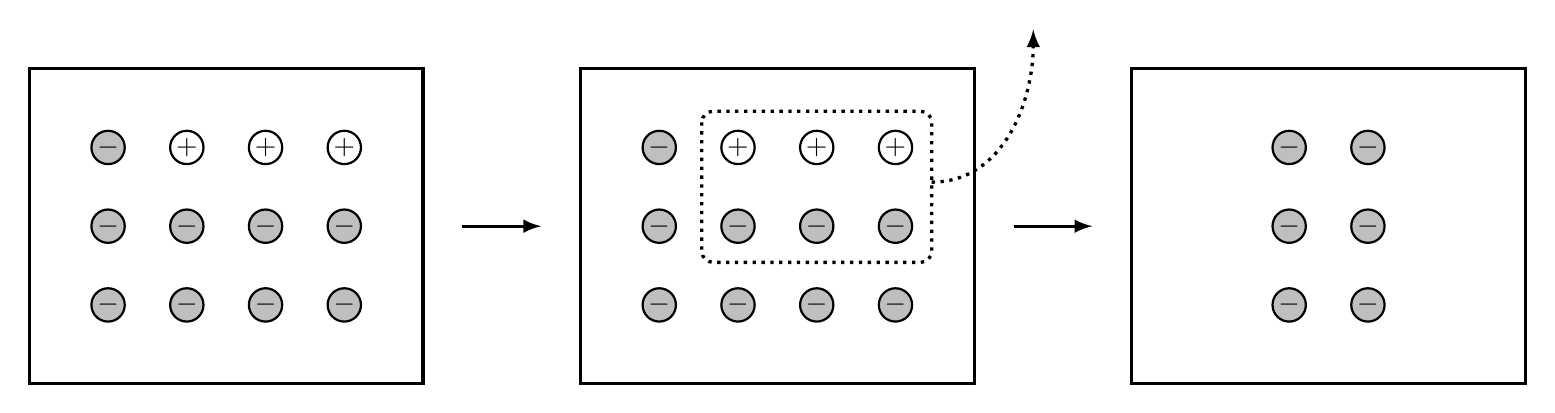
\begin{tikzpicture}[
	scale=1.0,
	circleA/.style={thick,draw,circle, inner sep=.65pt, fill=gray!50},%%set style for circles
	circleB/.style={thick,draw,circle, inner sep=.65pt,fill=white}
]
	\def\Ht{4};
	\def\Wt{5};
	\def\cirA{$-$};
	\def\cirB{$+$};
	
	\begin{scope}[shift ={(0,0)}]
		\node[circleA] at ({\Wt- \Wt+1},{\Ht-1}) {\cirA};%%1st row
		\node[circleB] at ({\Wt- \Wt+2},{\Ht-1}) {\cirB};
		\node[circleB] at ({\Wt- \Wt+3},{\Ht-1}) {\cirB};
		\node[circleB] at ({\Wt- \Wt+4},{\Ht-1}) {\cirB};
		\node[circleA] at ({\Wt- \Wt+1},{\Ht-2}) {\cirA};%%2nd row
		\node[circleA] at ({\Wt- \Wt+2},{\Ht-2}) {\cirA};
		\node[circleA] at ({\Wt- \Wt+3},{\Ht-2}) {\cirA};
		\node[circleA] at ({\Wt- \Wt+4},{\Ht-2}) {\cirA};
		\node[circleA] at ({\Wt- \Wt+1},{\Ht-3}) {\cirA};%%3rd row
		\node[circleA] at ({\Wt- \Wt+2},{\Ht-3}) {\cirA};
		\node[circleA] at ({\Wt- \Wt+3},{\Ht-3}) {\cirA};
		\node[circleA] at ({\Wt- \Wt+4},{\Ht-3}) {\cirA};
		\draw[very thick] (0,0) rectangle (\Wt,\Ht);
		\draw[very thick,-latex] ({\Wt+.5},\Ht /2)--({\Wt+1.5},\Ht /2);
	\end{scope}
	
	\begin{scope}[shift ={({\Wt + 2},0)}] %%second block
		\node[circleA] at ({\Wt- \Wt+1},{\Ht-1}) {\cirA};%%1st row
		\node[circleB] (A) at ({\Wt- \Wt+2},{\Ht-1}) {\cirB};
		\node[circleB] at ({\Wt- \Wt+3},{\Ht-1}) {\cirB};
		\node[circleB] at ({\Wt- \Wt+4},{\Ht-1}) {\cirB};
		\node[circleA] at ({\Wt- \Wt+1},{\Ht-2}) {\cirA};%%2nd row
		\node[circleA] at ({\Wt- \Wt+2},{\Ht-2}) {\cirA};
		\node[circleA] at ({\Wt- \Wt+3},{\Ht-2}) {\cirA};
		\node[circleA] (B) at ({\Wt- \Wt+4},{\Ht-2}) {\cirA};
		\node[circleA] at ({\Wt- \Wt+1},{\Ht-3}) {\cirA};%%3rd row
		\node[circleA] at ({\Wt- \Wt+2},{\Ht-3}) {\cirA};
		\node[circleA] at ({\Wt- \Wt+3},{\Ht-3}) {\cirA};
		\node[circleA] at ({\Wt- \Wt+4},{\Ht-3}) {\cirA};
		\draw[very thick, rounded corners, dotted] ($(A.north west)+(-0.3,0.3)$)  rectangle ($(B.south east)+(0.3,-0.3)$); %%draws box around nodes with corners(A) and (B)
		\draw[very thick,-latex,dotted] ($(B.north east)+(0.3,.4)$) to[out=0,in=-90] ({\Wt+.75},{\Ht+.5}); %in/out specifies in/out arrow angle
		\draw[very thick] (0,0) rectangle (\Wt,\Ht);
		\draw[very thick,-latex] ({\Wt+.5},\Ht /2)--({\Wt+1.5},\Ht /2);
	\end{scope}

	\begin{scope}[shift ={({2*(\Wt + 2)},0)}] %%third block
		%\node[circleA] at ({\Wt- \Wt+1},{\Ht-1}) {\cirA};%%1st row
		\node[circleA] at ({\Wt- \Wt+2},{\Ht-1}) {\cirA};
		\node[circleA] at ({\Wt- \Wt+3},{\Ht-1}) {\cirA};
		%\node[circlea] at ({\Wt- \Wt+4},{\Ht-1}) {\cirA};
		%\node[circleA] at ({\Wt- \Wt+1},{\Ht-2}) {\cirA};%%2nd row
		\node[circleA] at ({\Wt- \Wt+2},{\Ht-2}) {\cirA};
		\node[circleA] at ({\Wt- \Wt+3},{\Ht-2}) {\cirA};
		%\node[circleA] at ({\Wt- \Wt+4},{\Ht-2}) {\cirA};
		%\node[circleA] at ({\Wt- \Wt+1},{\Ht-3}) {\cirA};%%3rd row
		\node[circleA] at ({\Wt- \Wt+2},{\Ht-3}) {\cirA};
		\node[circleA] at ({\Wt- \Wt+3},{\Ht-3}) {\cirA};
		%\node[circleA] at ({\Wt- \Wt+4},{\Ht-3}) {\cirA};
		\draw[very thick] (0,0) rectangle (\Wt,\Ht);
		%\draw[very thick,-latex] ({\Wt+.5},\Ht /2)--({\Wt+1.5},\Ht /2);
	\end{scope}
	%\draw[help lines] (0,0) grid (\Wt,\Ht); %for location help
\end{tikzpicture}\end{center}
\end{figure}
\noindent Which of the following addition sentences represent the
model shown?

\begin{enumerate}
\item  \ans $-9x+3x=-6x$
\item $-12x+6x=-6x$
\item $12x-(-6x)=-6x$
\item $-4x+(-2x)=-6x$\yspace \vfill
\end{enumerate}
\item \questInd 
\begin{figure}[H]
\begin{center}
\[
12,14,15,16,19,20,20,20,22,23,23,25,31,31,32,33,35
\]
\end{center}
\end{figure}
\noindent The list shows the ages of people at Mrs. Bings' birthday
party. Which of the following statements about the ages must be true?

\begin{enumerate}
\item The mode is 22 years.
\item  \ans The median is 22 years.
\item  \ans The mean is 23 years.
\item The range is 42 years.\yspace \vfill
\end{enumerate}
\item \questMulti Which of the following is an algebraic equation?

\begin{enumerate}
\item $\frac{\sqrt{2x}+3y}{5}$
\item  \ans $\sqrt{2}x-3=5$
\item $2(3-2)=5\div(3+\sqrt{2})$
\item $5+2-\frac{10}{3}$\yspace \vfill
\end{enumerate}
\item \questMulti Which of the following is equivalent to $\frac{1}{3}\div9$

\begin{enumerate}
\item $\frac{1}{3}\times\frac{9}{1}$
\item  \ans $\frac{1}{3}\times\frac{1}{9}$
\item $\frac{3}{1}\times\frac{9}{1}$
\item $\frac{3}{1}\times\frac{1}{9}$\yspace \vfill
\end{enumerate}
\item \questMultiPic 
\begin{figure}[H]
\begin{center}%
\begin{tabular}{|c|>{\centering}m{4cm}|c|}
\hline 
\textbf{Term} & \textbf{Figure(s)} & \multirow{1}{*}{\textbf{Lines}}\tabularnewline
\hline 
1 & \begin{tikzpicture}[
scale=1.0,
shapeA/.style={regular polygon, regular polygon sides=5,very thick,draw, minimum size=15pt}, %%set style for shape A
shapeB/.style={cross,rotate=90,very thick,draw, minimum size=15pt} %%set style for shape A
]
\matrix[row sep=0pt,column sep=5pt] {
\node[shapeA] {};& 
\node[shapeB,white] {};&
\node[shapeA,white] {};&
\node[shapeB,white] {};&
\node[shapeA,white] {};\\
};
\end{tikzpicture} & 5\tabularnewline
\hline 
2 & 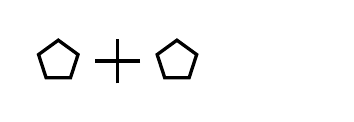
\begin{tikzpicture}[
scale=1.0,
shapeA/.style={regular polygon, regular polygon sides=5,very thick,draw, minimum size=15pt}, %%set style for shape A
shapeB/.style={cross,rotate=90,very thick,draw, minimum size=15pt} %%set style for shape A
]
\matrix[row sep=0pt,column sep=5pt] {
\node[shapeA] {};& 
\node[shapeB] {};&
\node[shapeA] {};&
\node[shapeB,white] {};&
\node[shapeA,white] {};\\
};
\end{tikzpicture} & 12\tabularnewline
\hline 
3 & 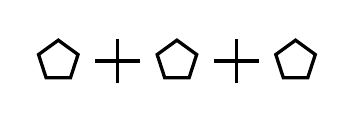
\begin{tikzpicture}[
scale=1.0,
shapeA/.style={regular polygon, regular polygon sides=5,very thick,draw, minimum size=15pt}, %%set style for shape A
shapeB/.style={cross,rotate=90,very thick,draw, minimum size=15pt} %%set style for shape A
]
\matrix[row sep=0pt,column sep=5pt] {
\node[shapeA] {};& 
\node[shapeB] {};&
\node[shapeA] {};&
\node[shapeB] {};&
\node[shapeA] {};\\
};
\end{tikzpicture} & 19\tabularnewline
\hline 
$\vdots$ & $\vdots$ & $\vdots$\tabularnewline
\hline 
\end{tabular}\end{center}
\end{figure}
\noindent In the sequence of figures shown in the table above, the
first term is made of a single shape and each successive term is made
by adding one shape as indicated by the pattern. 5 line segments are
needed to form a pentagon, and 2 line segments are needed to form
each cross. Which of the following expression can be used to find
the number of line segments needed to form the $n^{\mbox{th}}$ term
in each sequence of figures?

\begin{enumerate}
\item $n+7$
\item  \ans $7n-2$
\item $n^{2}+3$
\item $(n+1)^{2}-4$\yspace \vfill
\end{enumerate}
\item \questMulti The digit 1 is in what place in the number 6.283185?

\begin{enumerate}
\item Hundredths place
\item Thousandths place
\item  \ans Ten-thousandths place
\item Hundred-thousandths place\yspace \vfill
\end{enumerate}
\item \questMulti Roger the rabbit left his rabbit hole at 2:55 P.M., and
it took him $\frac{2}{3}$ of an hour to get to the forest. At what
time did Roger get to the forest?

\begin{enumerate}
\item 3:25 P.M.
\item  \ans 3:35 P.M.
\item 3:45 P.M.
\item 3:55 P.M.\yspace \vfill
\end{enumerate}
\item \questMulti Harry the magician agreed to pay his agent 30\% of the
ticket sales from his shows. If the ticket sales from Harry's last
show was \$201.30, how much does Harry owe his agent?

\begin{enumerate}
\item \$6.04
\item  \ans \$60.39
\item \$67.10
\item \$603.9\yspace \vfill
\end{enumerate}
\item \questMulti In the \emph{xy-}plane, point \emph{R} has coordinates
$(3,2)$ and point \emph{S }has coordinates $(8,2)$. Which of the
following could be the coordinates for point \emph{T }so that the
area of triangle \emph{RST }is equal to 15 square units?

\begin{enumerate}
\item  \ans $(6,8)$
\item $(6,4)$
\item $(8,4)$
\item $(3,6)$\yspace \vfill
\end{enumerate}
\item \questMultiPic 
\begin{figure}[H]
\begin{center}%%%%graph with grid and labels 
\renewcommand{\xmax}{5} 
\renewcommand{\xmin}{0} 
\renewcommand{\xstep}{0} %must be xmin+n 
\renewcommand{\ymax}{550} 
\renewcommand{\ymin}{0} 
\renewcommand{\ystep}{0} %must be ymin+n %%%%%%% 
\begin{tikzpicture}  
\begin{axis}[ 	
	height=8cm,  	
	width=8cm,  	
	axis lines=middle, 	
	ymax=\ymax, ymin=\ymin,	
	xmax=\xmax, xmin=\xmin,
	grid=both,
	minor tick num=1,%%gridlines between tickmarks
	xtick={0,1,2,3,4,...,12}, 	
	ytick={0,100,200,...,500}, 	
	%every axis x label/.append style={anchor=west},  	
	%every axis y label/.append style={anchor=south},	 	
	x label style={at={(axis description cs:0.5,-0.15)},anchor=north},
	y label style={at={(axis description cs:-0.25,0.5)},rotate=90,anchor=south},
	axis line style={thick, shorten >=-10pt, shorten <=-5pt},%%lengthen axis line to grid	
	xlabel={\textSize Number of Days}, 	
	ylabel={\textSize Number of Pages Written}, 	
	%clip=false, %doesn't clip outside graph 	
	] 	
	\addplot[-latex,domain=\xmin:\xmax-.25,samples=100,draw=black,thick]{125*x} [yshift=5pt]  		node[pos=0.5,above] {$$}; 
	\node[circle,fill,inner sep=1.5pt] at (axis cs:1,125) {};
	\node[circle,fill,inner sep=1.5pt] at (axis cs:2,250) {};
	\node[circle,fill,inner sep=1.5pt] at (axis cs:3,375) {};
	\node[circle,fill,inner sep=1.5pt] at (axis cs:4,500) {};

\end{axis} 
\end{tikzpicture}\end{center}
\end{figure}
 \noindent Stephen Koontz is writing a 750-page novel at a constant
rate. The graph shows the number of pages, \emph{y}, he has written
after \emph{x }days of writing. Assuming he continues writing as the
same rate, how many days will it him to finish writing the novel?

\begin{enumerate}
\item 4
\item  \ans 6
\item 8
\item 10\yspace \vfill
\end{enumerate}
\item \questInd 
\begin{figure}[H]
\begin{center}$2,4,8,\dots$\end{center}
\end{figure}
\noindent The first three terms of a sequence are shown. Which of
the following mathematical relationships could describe the terms
of the sequence?\\
\\
Select \textbf{all} that apply. 

\begin{enumerate}
\item  \ans The first term is 2. Each subsequent term of the sequence
is obtained by multiplying a constant by the preceding term.
\item The first term is 2. Each subsequent term of the sequence is obtained
by adding a constant to the preceding term.
\item The first term is 2. Each subsequent term of the sequence is obtained
by squaring the previous term. 
\item  \ans The first term is 2. Each subsequent term of the sequence
is obtained by adding the preceding term and a quantity that increases
by 2 with each new term. 
\item  \ans The first term is 2. Each subsequent term of the sequence
is obtained by squaring the previous term and subtracting a constant
that increases by 8 with each new term. \yspace \vfill
\end{enumerate}
\item \questMulti $x$ and $y$ are digits in some number, and $x$ represents
$10^{3}$times what $y$ represents. Which of the following could
be the place of $x$ and $y$?

\begin{enumerate}
\item $x$ is the thousandths place, and $y$ is the ones place.
\item $x$ is the tenths place, and $y$ is the hundreds place.
\item $x$ is the tens place, and $y$ is in the thousandths place.
\item  \ans $x$ is in the tens place, and $y$ is in the hundredths place.
\yspace \vfill
\end{enumerate}
\item \questMulti At a local high-school with 30 paid employees, one employee
has an annual salary of \$135 thousand, three employees have an annual
salary of \$50 thousand each, and the remaining have annual salaries
of \$25 thousand each. Which of the following best represents a typical
employee's annual salary?

\begin{enumerate}
\item Mean
\item  \ans Median
\item Mid-range
\item Range\yspace \vfill
\end{enumerate}
\item \questMultiPic 
\begin{figure}[H]
\begin{center}$\left(3z-2z+1\right)-\left(-7z+8z-1\right)$\end{center}
\end{figure}
 \noindent Which of the following is equivalent to the expression
shown?

\begin{enumerate}
\item  \ans 2
\item 0
\item $2z+2$
\item $2z$\yspace \vfill
\end{enumerate}
\item \questMultiPic 
\begin{figure}[H]
\begin{center}1,364,520.79\end{center}
\end{figure}
 \noindent In the number shown above, the value represented by the
digit $4$ is $4\times c$, where $c$ is a constant. Which of the
following equals $c$?

\begin{enumerate}
\item $10^{2}$
\item  \ans $10^{3}$
\item $10^{4}$
\item $10^{5}$\yspace \vfill
\end{enumerate}
\item \questMulti Which of the following statements must be true about
the two non-obtuse angles of an obtuse triangle?

\begin{enumerate}
\item Both angles are obtuse.
\item One angle is acute and one is angle is obtuse.
\item  \ans Both angles are acute.
\item The angles are congruent.\yspace \vfill
\end{enumerate}
\item \questMultiPic 
\begin{figure}[H]
\begin{center}$-5(x-2)\leq20$\end{center}
\end{figure}
 \noindent Which of the following inequalities is equivalent to the
inequality shown?

\begin{enumerate}
\item $x\leq-2$
\item $x\leq2$
\item  \ans $x\geq-2$
\item $x\geq2$\yspace \vfill
\end{enumerate}
\item \questMultiPic 
\begin{figure}[H]
\begin{center}$6+18\div2\times\left(5-2\right)$\end{center}
\end{figure}
 \noindent Which of the following is equivalent to the expression
shown?

\begin{enumerate}
\item 4
\item 9
\item  \ans 33
\item 36\yspace \vfill
\end{enumerate}
\item \questMulti Which list of numbers is ordered from least to greatest?

\begin{enumerate}
\item $\frac{13}{22}$, $0.44$, $\frac{3}{5}$, $0.\bar{44}$
\item  \ans $0.44$, $0.\bar{44}$, $\frac{13}{22}$, $\frac{3}{5}$
\item $\frac{3}{5}$, $\frac{13}{22}$, $0.44$, $0.\bar{44}$, 
\item $0.\bar{44}$, $0.44$, $\frac{13}{22}$, $\frac{3}{5}$\yspace \vfill
\end{enumerate}
\item \questFill A container in the shape of a cube is completely filled
with 64 number cubes. Each number cube has an edge that is $\frac{3}{4}$
of a foot long. Find the volume, in cubic feet, of the container.
\begin{figure}[H]
\begin{center}


\begin{tikzpicture}[scale=1]
	\draw[ultra thick, blue!25!black] (0,0) rectangle (3,1) node[pos=.5] {\answer{27}};	
\end{tikzpicture}

\end{center}
\end{figure}
\yspace \vfill
\item \questMulti A banker evaluates the data in spreadsheet with records
of total investments each day for one month. The banker deletes the
greatest and smallest investment for the month from the spreadsheet.
How is the data set most likely affected by removing this action?

\begin{enumerate}
\item The mean and median of the data set will change, but the range will
stay the same.
\item The median and range of the data set will change, but the mean will
stay the same.
\item  \ans The mean and range of the data set will change, but the median
will stay the same.
\item The median, mean, and range of the data set will all change.\yspace \vfill
\end{enumerate}
\item \questMulti Determine which of the following two numbers estimates
the number 1,409.147351 to the nearest tenth and to the nearest ten-thousandths,
respectively? 

\begin{enumerate}
\item 1,409.1 and 1,409.1473
\item  \ans 1,409.1 and 1,409.1474
\item 1,409.2 and 1,409.1473
\item 1,409.2 and 1,409.1474\yspace \vfill
\end{enumerate}
\item \questMulti James bought a new kayak with a price tag of \$899.99.
He also has to pay sales tax rate at a rate 0f 6.9\%. Determine which
of the following proportions can be used to find the amount of sales
tax, $t$, in dollars, for the new kayak?

\begin{enumerate}
\item $\dfrac{6.9}{899.99}=\dfrac{t}{100}$
\item $\dfrac{6.9}{899.99}=\dfrac{100}{t}$
\item  \ans $\dfrac{6.9}{100}=\dfrac{t}{899.99}$
\item $\dfrac{6.9}{100}=\dfrac{899.99}{t}$\yspace \vfill
\end{enumerate}
\item \questMultiPic 
\begin{figure}[H]
\begin{center}$\left(x+1\right)\left(y-2\right)+\left(y+2\right)\left(x+1\right)$\end{center}
\end{figure}
 \noindent Which of the following expressions is equivalent to the
expression shown?

\begin{enumerate}
\item $2y$
\item $\left(x+1\right)$
\item $2\left(x+1\right)$
\item  \ans $2y\left(x+1\right)$\yspace \vfill
\end{enumerate}
\item \questMulti Tess made 453,592 milligrams of pasta. Which of the following
represents the amount of pasta, in grams, that Tess made?

\begin{enumerate}
\item 45.3592
\item  \ans 453.592
\item 4535.92
\item 453,592,000\yspace \vfill
\end{enumerate}
\item \questMulti $3\dfrac{3}{4}\%$ is equivalent to which of the following
numbers?

\begin{enumerate}
\item $3.75$
\item $0.375$
\item  \ans $0.0375$
\item $0.00375$\yspace \vfill
\end{enumerate}
\item \questInd 
\begin{figure}[H]
\begin{center}$5x^{2}+7y^{2}-13xy^{2}+4x^{2}y+2$\end{center}
\end{figure}
 \noindent Which THREE of the following statements are correct about
the given algebraic expression?

\begin{enumerate}
\item The coefficients are 5, 7, -13, and 4
\item  \ans The variables are $x$ and $y$.
\item There are like terms.
\item  \ans There are five terms.
\item  \ans The degree of the expression is 3.\yspace \vfill
\end{enumerate}
\item \questMultiPic 
\begin{figure}[H]
\begin{center}%\renewcommand*{\arraystretch}{2}%
\begin{tabular}{|c|>{\centering}m{3cm}|}
\hline 
Label & Probability\tabularnewline
\hline 
1 & \vspace{10pt}$\frac{1}{4}$\vspace{10pt}\tabularnewline
\hline 
2 & \vspace{10pt}$\dfrac{3}{8}$\vspace{10pt}\tabularnewline
\hline 
3 & \vspace{10pt}$x$\vspace{10pt}\tabularnewline
\hline 
4 & \vspace{10pt}$\dfrac{1}{16}$\vspace{10pt}\tabularnewline
\hline 
\end{tabular}\end{center}
\end{figure}
 \noindent A spinner is divided into 16 congruent sections. Each
section is labeled as either 1, 2, 3, or 4. The table shows the theoretical
probability of landing on a number when spinning the spinner one time.
How many sections are labeled 3?

\begin{enumerate}
\item 2
\item 4
\item  \ans 5
\item 11\yspace \vfill
\end{enumerate}
\item \questMulti Square A has an area of 1 square meter. The length of
each side of square B is 1 meter greater than the length of each side
of square A. The area of square B is how many times the area of square
A?

\begin{enumerate}
\item 1 times
\item 2 times
\item  \ans 4 times
\item 8 times\yspace \vfill
\end{enumerate}
\item \questMulti Chef is making 4 chocolate cakes for a Kermit's birthday
party. Each cake requires $2\dfrac{1}{4}$ cups of flour and $3\dfrac{1}{2}$
cups of chocolate syrup. Which of the following is the best estimate
of the total amount of flour and chocolate syrup necessary to make
the cakes?

\begin{enumerate}
\item Less than 20
\item  \ans Between 20 and 24 cups. 
\item Between 24 and 27
\item More than 27\yspace \vfill
\end{enumerate}
\item \questMultiPic 
\begin{figure}[H]
\begin{center}$-d+5r$\end{center}
\end{figure}
 \noindent What is the value of the expression shown when $d=2$
and $r=-3$?

\begin{enumerate}
\item  \ans $-17$
\item $-13$
\item $13$
\item $17$\yspace \vfill
\end{enumerate}
\item \questMultiPic 
\begin{figure}[H]
$\left\{ 7,\,\,9,\,\,-1,\,\,2,\,\,5,\,\,10,\,\,8,\,\,2,\,\,7,\,\,0,\,\,3,\,\,7,\,\,6\right\} $
\end{figure}
\begin{figure}[H]
\begin{center}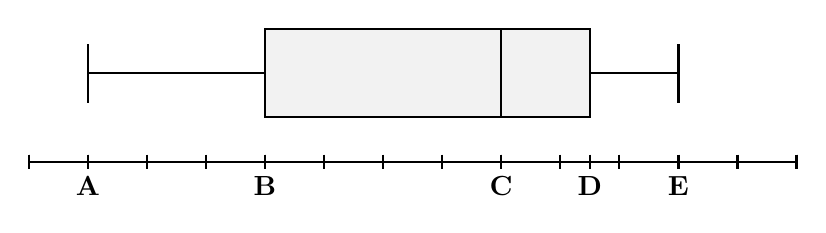
\begin{tikzpicture} [scale=.75, thick]   	
	\def\Xmin{-2} %%sets values for boxplot 	
	\def\Xmax{11} 	
	\def\Min{-1} 	
	\def\QrtA{2} 	
	\def\QrtB{6} 	
	\def\QrtC{7.5} 	
	\def\Max{9} 

	\filldraw[fill=gray!10] (\QrtA,-.25) rectangle (\QrtC,1.25);   	
	\draw (\QrtB,-.25)--(\QrtB,1.25); %node[above]{Median};   	
	\draw (\QrtC,0.5)--(\Max,0.5); %vandret linie til max   	
	\draw (\QrtA,0.5)--(\Min,0.5); %vandret linie til min 	%%T-cap line ends
	\draw (\Max,0.0)--(\Max,1); %node[above]{\small maximum}; 
	\draw (\Min,0.0)--(\Min,1); %node[above]{\small minimum};    
	\draw [postaction={draw, decoration=ticks, segment length=.75 cm, decorate}] (\Xmin,-1) -- (\Xmax,-1); %set to scale, draws x-axis
	
	\foreach \tick in {\Xmin,\Min,\QrtA,\QrtB,\QrtC, \Xmax}
		\draw [postaction={draw, decoration=ticks, decorate}] (\tick, -1); 		%node [below=1pt] {\tick};
	\node at (\Min,-1) [below=1.5pt] {\textbf{A}};
	\node at (\QrtA,-1) [below=1.5pt] {\textbf{B}};
	\node at (\QrtB,-1) [below=1.5pt] {\textbf{C}};
	\node at (\QrtC,-1) [below=1.5pt] {\textbf{D}};
	\node at (\Max,-1) [below=1.5pt] {\textbf{E}};

\end{tikzpicture}\end{center}

\caption*{\textbf{Note:} Figure not drawn to scale.}
\end{figure}
 \noindent The list above shows the number of days missed this year
by each of 13 students in a class. The data is summarized in the provided
boxplot. What is the value of B on the boxplot?

\begin{enumerate}
\item  \ans 2
\item 3
\item 5
\item 6\yspace \vfill
\end{enumerate}
\item Alisha's cat eats $\frac{1}{2}$ of a 10 pound bag of cat food every
day. How many 10 pound bags must she buy to feed her cat for one week?

\begin{enumerate}
\item 3
\item 3.5
\item  \ans 4
\item 4.5\yspace \vfill
\end{enumerate}
\item \questMultiPic 
\begin{figure}[H]
\begin{center}\begin{tikzpicture}[scale=0.75] %%scale is 1 inch=5/21         	
	\tkzDefPoint(0,0){A}         
	\tkzDefPoint(10,0){B}         
	\tkzDefPoint(10,36*5/21){C}         
	\tkzDefPoint(5,36*5/21){D}         
	\tkzDefPoint(5,12*5/21){E}         
	\tkzDefPoint(0,12*5/21){F}         
	\tkzDefPoint[yshift=16pt](0,36*5/21){G} %%streches view box                 	
	%\tkzLabelPoints[](A,B,C,D,E,F)          
	\tkzDrawPolygon[thick](A,B,C,D,E,F)         
	\tkzMarkRightAngle[size=.35](F,A,B)         
	\tkzMarkRightAngle[size=.35](A,B,C)         
	\tkzMarkRightAngle[size=.35](B,C,D)         
	\tkzMarkRightAngle[size=.35](C,D,E)         
	\tkzMarkRightAngle[size=.35](B,C,D)         
	\tkzMarkRightAngle[size=.35](E,F,A)                  

	%%dimension labels%%         
	
	\def\Yshift{13} %Vertical shift of dim labels      
	\def\Xshift{22.75} %hortizontal shift of dim labels
	\def\Diff{6} %distance of dim labels from object                 
	
	\foreach \Nodo in {F,E,D,C} %%drwas end lines for above dimensiona
		\draw ([yshift=\Yshift-\Diff]\Nodo) -- ([yshift=\Yshift+\Diff]\Nodo);
	\foreach \A in {F} %%draw dim line
		\foreach \B in {E}
			\draw[<->,>=latex] ([yshift=\Yshift]\A) -- node[fill=white] {$1.75$\,in} ([yshift=\Yshift]\B);         
	\foreach \A in {D} %%draw dim line             
		\foreach \B in {C}             
			\draw[<->,>=latex] ([yshift=\Yshift]\A) -- node[fill=white] {$21$\,in} ([yshift=\Yshift]\B);                  
			
	\foreach \Nodo in {A,F} %%drwas end lines for left dimensions             
		\draw ([xshift=-\Diff]\Nodo) -- ([xshift=-2*\Xshift+\Diff]\Nodo);         		
	\foreach \A in {A} %%draw dim line             
		\foreach \B in {F}          		
			\draw[<->,>=latex] ([xshift=-\Xshift]\A) -- node[fill=white] {$1$\,ft} ([xshift=-\Xshift]\B);                                
	
	\foreach \Nodo in {B,C} %%drwas end lines for right dimensions             	
		\draw ([xshift=\Diff]\Nodo) -- ([xshift=2*\Xshift-\Diff]\Nodo);         		
	\foreach \A in {B} %%draw dim line           
		\foreach \B in {C}      
			\draw[<->,>=latex] ([xshift=\Xshift]\A) -- node[fill=white] {$3$\,yd} ([xshift=\Xshift]\B);                    

\end{tikzpicture}\end{center}
\end{figure}
 \noindent Find the area of the shown polygon. 

\begin{enumerate}
\item 25.75 square inches
\item 165.5 square inches
\item 777 square inches
\item  \ans 2289 square inches\yspace \vfill
\end{enumerate}
\item \questMultiPic 
\begin{figure}[H]
\[
17x^{3}+2y^{2}+5x+17y+30x^{3}-14y^{3}
\]
\end{figure}
 \noindent Which of the following shows all like terms of the expression
above?

\begin{enumerate}
\item $2y^{2}$, $17y$, and $-14y^{3}$
\item $17x^{3}$ and $17y$
\item $17x^{3}$, $30x^{3}$, and $-14y^{3}$
\item  \ans $17x^{3}$ and $30x^{3}$\yspace \vfill
\end{enumerate}
\item \questMultiPic 
\begin{figure}[H]
\begin{tabular}{|c|>{\centering}m{3cm}|}
\hline 
Job & \vspace{2pt}Time\vspace{2pt}\tabularnewline
\hline 
Cutting Hair & \vspace{2pt}15 minutes\vspace{2pt}\tabularnewline
\hline 
Tutoring Math & \vspace{2pt}8 minutes\vspace{2pt}\tabularnewline
\hline 
Mowing Lawns & \vspace{2pt}20 minutes\vspace{2pt}\tabularnewline
\hline 
\end{tabular}
\end{figure}
 \noindent The table shows the time it takes Lucinda to earn \$10
while working each of the three listed jobs. If Lucinda cuts hair
for 30 minutes, tutors math for 20 minutes, and then mows lawns for
15 minutes, how much money would she have earned?

\begin{enumerate}
\item \$27.50
\item \$40.00
\item  \ans \$52.50
\item \$62.5\yspace \vfill
\end{enumerate}
\item \questMultiPic 
\begin{figure}[H]
\[
2\times4+5\times4
\]
\end{figure}
 \noindent The expression shows the result when the distributive
property of multiplication over addition is applied to which of the
following expressions?

\begin{enumerate}
\item $8+20$
\item  \ans $\left(2+5\right)\times4$
\item $2+2+2+2+5+5+5+5$
\item $\left(5\times4\right)+\left(2\times4\right)$\yspace \vfill
\end{enumerate}
\item \questMultiPic 
\begin{figure}[H]
\[
4-2x\geq-\frac{1}{3}x-1
\]
\end{figure}
 \noindent Which of the following is the graph of the solutions to
the inequality shown?

\begin{enumerate}
\item %
\begin{minipage}[c][1\totalheight][t]{1\columnwidth}%
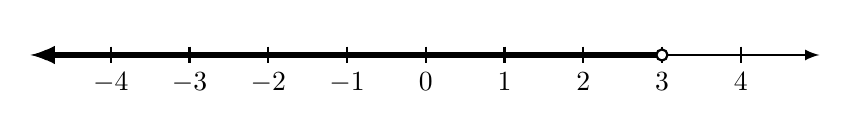
\begin{tikzpicture}[scale=1.0]     
	\def\Min{-4};     
	\def\Max{4};     
	\def\ptA{3}; %first point for line     
	\def\ptB{\Min -1.02}; %second pt for line          
	
	\draw[thick,latex-latex] (\Min-1,0) -- (\Max+1,0) ;     
	\foreach \x in  {\Min,...,\Max}     
		\draw[thick,shift={(\x,0)},color=black] (0pt,3pt) -- (0pt,-3pt);     
	\foreach \x in {\Min,...,\Max}     
		\draw[shift={(\x,0)},color=black] (0pt,0pt) -- (0pt,-3pt) node[below] {$\x$};          	\draw[shift={(0,0)},color=black] (0pt,0pt) -- (0pt,3pt) node[above] {$$}; %%for vertical spacing
	
	\draw[line width=2.0pt,-latex] (\ptA,0) -- (\ptB,0);%%line for interval/inequality         
		%\path [draw=black, fill=black] (\ptA,0) circle (2pt);         
		\path [draw=black, fill=white, thick] (\ptA,0.0) circle (2pt);
\end{tikzpicture}%
\end{minipage}
\item %
\begin{minipage}[c][1\totalheight][t]{1\columnwidth}%
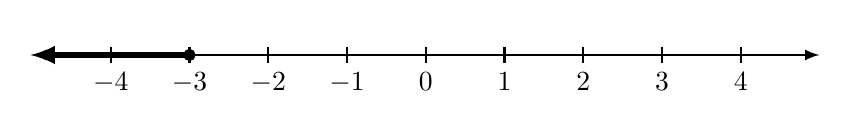
\begin{tikzpicture}[scale=1.0]     
	\def\Min{-4};     
	\def\Max{4};     
	\def\ptA{-3}; %first point for line     
	\def\ptB{\Min -1.02}; %second pt for line          
	
	\draw[thick,latex-latex] (\Min-1,0) -- (\Max+1,0) ;     
	\foreach \x in  {\Min,...,\Max}     
		\draw[thick,shift={(\x,0)},color=black] (0pt,3pt) -- (0pt,-3pt);     
	\foreach \x in {\Min,...,\Max}     
		\draw[shift={(\x,0)},color=black] (0pt,0pt) -- (0pt,-3pt) node[below] {$\x$};          	\draw[shift={(0,0)},color=black] (0pt,0pt) -- (0pt,3pt) node[above] {$$}; %%for vertical spacing
	
	\draw[line width=2.0pt,-latex] (\ptA,0) -- (\ptB,0);%%line for interval/inequality         
		\path [draw=black, fill=black] (\ptA,0) circle (2pt);         
		%\path [draw=black, fill=white, thick] (\ptB,0.0) circle (2pt);
\end{tikzpicture}%
\end{minipage}
\item  \ans %
\begin{minipage}[c][1\totalheight][t]{1\columnwidth}%
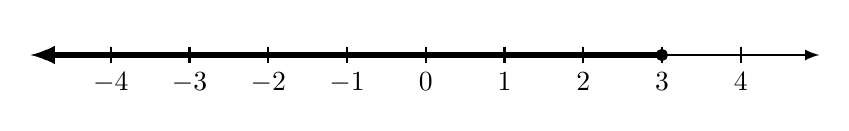
\begin{tikzpicture}[scale=1.0]     
	\def\Min{-4};     
	\def\Max{4};     
	\def\ptA{3}; %first point for line     
	\def\ptB{\Min -1.02}; %second pt for line          
	
	\draw[thick,latex-latex] (\Min-1,0) -- (\Max+1,0) ;     
	\foreach \x in  {\Min,...,\Max}     
		\draw[thick,shift={(\x,0)},color=black] (0pt,3pt) -- (0pt,-3pt);     
	\foreach \x in {\Min,...,\Max}     
		\draw[shift={(\x,0)},color=black] (0pt,0pt) -- (0pt,-3pt) node[below] {$\x$};          	\draw[shift={(0,0)},color=black] (0pt,0pt) -- (0pt,3pt) node[above] {$$}; %%for vertical spacing
	
	\draw[line width=2.0pt,-latex] (\ptA,0) -- (\ptB,0);%%line for interval/inequality         
		\path [draw=black, fill=black] (\ptA,0) circle (2pt);         
		%\path [draw=black, fill=white, thick] (\ptB,0.0) circle (2pt);
\end{tikzpicture}%
\end{minipage}
\item %
\begin{minipage}[c][1\totalheight][t]{1\columnwidth}%
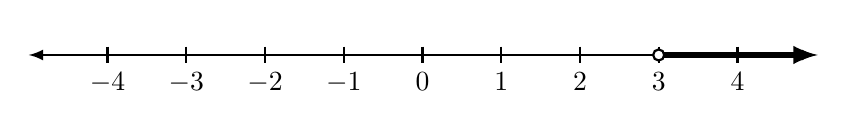
\begin{tikzpicture}[scale=1.0]     
	\def\Min{-4};     
	\def\Max{4};     
	\def\ptA{3}; %first point for line     
	\def\ptB{\Max +1.02}; %second pt for line          
	
	\draw[thick,latex-latex] (\Min-1,0) -- (\Max+1,0) ;     
	\foreach \x in  {\Min,...,\Max}     
		\draw[thick,shift={(\x,0)},color=black] (0pt,3pt) -- (0pt,-3pt);     
	\foreach \x in {\Min,...,\Max}     
		\draw[shift={(\x,0)},color=black] (0pt,0pt) -- (0pt,-3pt) node[below] {$\x$};          	\draw[shift={(0,0)},color=black] (0pt,0pt) -- (0pt,3pt) node[above] {$$}; %%for vertical spacing
	
	\draw[line width=2.0pt,-latex] (\ptA,0) -- (\ptB,0);%%line for interval/inequality         
		%\path [draw=black, fill=black] (\ptA,0) circle (2pt);         
		\path [draw=black, fill=white, thick] (\ptA,0.0) circle (2pt);
\end{tikzpicture}%
\end{minipage}\yspace \vfill
\end{enumerate}
\item \questMulti Which of the following list all of the factors of 36

\begin{enumerate}
\item 2, 3
\item 3, 4, 6, 9
\item 2, 3, 4, 6, 9, 12, 18
\item  \ans 1, 2, 3, 4, 6, 9, 12, 18, 36\yspace \vfill
\end{enumerate}
\item \questMultiPic 
\begin{figure}[H]
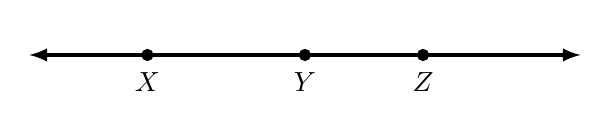
\begin{tikzpicture}[scale=1.0]     
	\def\Min{0};     
	\def\Max{6};     
	\def\ptA{1}; %first pt     
	\def\ptB{3}; %second pt     
	\def\ptC{4.5};           
	
	\draw[very thick,latex-latex] (\Min-.5,0) -- (\Max+.5,0) ;          
	\foreach \x/\y in { \ptA/X,\ptB/Y,\ptC/Z}         
		\draw[draw=black,fill=black] (\x,0) circle (2pt) node[yshift=-3pt,below] {$\y$}; %%labels pts
   \draw[shift={(0,0)},color=black] (0pt,0pt) -- (0pt,0pt) node[yshift=3pt,above] {$ $}; %%for vertical spacing
\end{tikzpicture}
\end{figure}
 \noindent Which of the following can be used to name the ray that
has endpoint $Z$ and goes in the direction of $X$ in the figure
shown?

\begin{enumerate}
\item $\overrightarrow{ZX}$ only
\item $\overrightarrow{ZY}$ only
\item  \ans $\overrightarrow{ZX}$ and $\overrightarrow{ZY}$
\item $\overrightarrow{ZX}$ and $\overrightarrow{XZ}$\yspace \vfill
\end{enumerate}
\item \questMulti The function $f\left(x\right)=-x^{2}+1$ is represented
by which of the following tables?

\begin{enumerate}
\item  \ans %
\begin{minipage}[c][1\totalheight][t]{1\columnwidth}%
\begin{tabular}{c|c}
$x$ & $f(x)$\tabularnewline
\hline 
-2 & -3\tabularnewline
0 & 1\tabularnewline
1 & 0\tabularnewline
4 & -15\tabularnewline
\end{tabular}%
\end{minipage}
\item %
\begin{minipage}[c][1\totalheight][t]{1\columnwidth}%
\begin{tabular}{c|c}
$x$ & $f(x)$\tabularnewline
\hline 
-2 & 5\tabularnewline
0 & 1\tabularnewline
1 & 0\tabularnewline
4 & -15\tabularnewline
\end{tabular}%
\end{minipage}
\item %
\begin{minipage}[c][1\totalheight][t]{1\columnwidth}%
\begin{tabular}{c|c}
$x$ & $f(x)$\tabularnewline
\hline 
-2 & 5\tabularnewline
0 & 1\tabularnewline
1 & 2\tabularnewline
4 & 17\tabularnewline
\end{tabular}%
\end{minipage}
\item %
\begin{minipage}[c][1\totalheight][t]{1\columnwidth}%
\begin{tabular}{c|c}
$x$ & $f(x)$\tabularnewline
\hline 
-2 & 5\tabularnewline
0 & 1\tabularnewline
1 & -1\tabularnewline
4 & -7\tabularnewline
\end{tabular}%
\end{minipage}\yspace \vfill
\end{enumerate}
\end{enumerate}
%%%%%%%%%%%%%%%old exam
\end{document}
